\chapter{Data Origin Authentication in the Quantum Networking Stack}
\label{chp:doa}

\begin{abstract}
Quantum networking protocols make use of classical communications to coordinate entanglement
generation and other tasks. In this chapter, we discuss the need for authentication of
classical messages exchanged at the quantum network stack level, with focus on concrete protocol
proposals. We then experimentally measure the overhead incurred by sending authenticated
classical messages through an authentication system that uses key material supplied by an
\acrshort{mdiqkd} system. We use this information to simulate the performance of a quantum link
whose protocol stack uses an authenticated classical channel, and compare that to existing
simulations of the same protocol stack. We find that message authentication overhead is not
detrimental to entanglement generation and to the fidelity of the entangled pairs.
\end{abstract}

\blfootnote{
This chapter is based on the article in preparation: \fullcite{abrahams_2023_doa_noprint}.

Contributions: J. S. Abrahams, \textbf{C. Delle Donne}, J. A. Slater and S. Wehner designed the
research. J. S. Abrahams researched and implemented \acrshortpl{mac}. P. Brussee, T. Middelburg and
R. C. Berrevoets prepared the authentication proxy. J. S. Abrahams and \textbf{C. Delle Donne}
prepared the framework to measure \acrshort{rtt} delays. J. S. Abrahams and \textbf{C. Delle Donne}
ran the simulations. J. S. Abrahams, \textbf{C. Delle Donne}, J. A. Slater and S. Wehner wrote the
manuscript with input from all authors. J. A. Slater and S. Wehner supervised the research. J. S.
Abrahams and \textbf{C. Delle Donne} contributed equally to this work.
}

\newpage

\lettrine{U}{p} until now, several proposals have been put forward as to how quantum networks should
be structured~\cite{van_meter_2013_repeaters, schoute_2016_shortcuts, joshi_2020_trusted}.
Researchers are also investigating how to abstract the complex physics of quantum network devices so
as to provide platform-independent services to the end user~\cite{dahlberg_2019_egp,
pirker_2019_quantum, illiano_2022_quantum} --- one very basic service would be the distribution of
entanglement between network nodes, that is, \emph{entanglement generation}. To coordinate this, and
other activities, proposals for a \emph{quantum network stack} have provided outlines of the layers
and the separation of responsibilities, as well as protocols to populate these
layers~\cite{dahlberg_2019_egp, kozlowski_2020_qnp}. Within the proposed stack, each layer makes use
of the service exposed by the layer below, and provides a higher-level service to the layer
above~\cite{dahlberg_2019_egp}. This stack is inspired by classical architectures like the
well-known TCP/IP network stack or the more generic \acrfull{osi} model, and is illustrated in
\cref{fig:functional-allocation}. Each layer and protocol within the quantum network stack makes use
of classical control messages, exchanged over a classical network, to coordinate the quantum
communication activities. These messages from the \emph{control protocols} form what we refer to as
the \emph{classical data plane} --- which lives alongside the \emph{quantum data plane}, in which
information encoded in quantum systems is transmitted.

\begin{figure}[b]
    \centering
    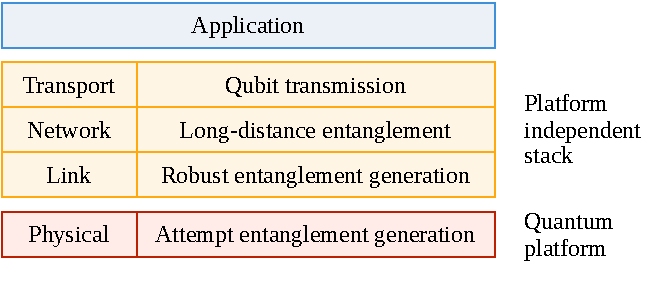
\includegraphics[width=0.6\linewidth]{figures/functional-allocation.pdf}
    \caption{
        Functional allocation of layers in a quantum network stack, adapted from
        Ref.~\cite{dahlberg_2019_egp}. The physical layer is quantum platform-dependent. The link
        layer provides platform-independent robust entanglement generation. All subsequent layers
        are therefore also platform independent, including the network and optionally transport
        layers which facilitate end-to-end entanglement between non-adjacent nodes. The application
        layer uses the services offered by the stack to perform quantum networking tasks.
    }
    \label{fig:functional-allocation}
\end{figure}

When designing control protocols for quantum networks, one should carefully estimate various key
performance indicators, such as their impact on the end-to-end latency of quantum services, such as
entanglement generation between network nodes. One obvious reason to assess the impact on latency,
is the fundamental aspect of quantum information which happens to impose strict constraints on
end-to-end latency: \emph{decoherence}. Storing quantum data reliably for extended periods of time
is non-trivial. Qubits have relatively short lifetimes, usually of the order of milliseconds, or at
best of a few seconds~\cite{abobeih_2018_one_sec, bradley_2019_one_min}. Therefore, not only can
high end-to-end latency affect the quality of the service offered by the network, but in some cases
it may result in no service at all. Classical processing and communication overhead must, thus, be
kept to a minimum, such that the generated entangled qubits can be used as quickly as possible.

On top of that, control messages must be transmitted in a secure manner for a quantum network to
function reliably. \textcite{satoh_2020_attacking} list forged classical messages as a general
concern for quantum networks. To prevent such forgeries, quantum network nodes may employ
\acrfull{doa} cryptography suites, to distinguish between genuine and fraudulent control messages.
\acrshort{doa} is performed using a secret that is shared between two parties. Then, a \acrfull{mac}
algorithm can produce a tag for each control message both at the sending and at the receiving end,
to verify that the message contents
%
\begin{inlinelist}
    \item were not altered and
    \item were produced by a party which owns the shared secret.
\end{inlinelist}
This process --- known as \emph{authentication} --- is illustrated in \cref{fig:mac-structure}.

\begin{figure}[t]
    \centering
    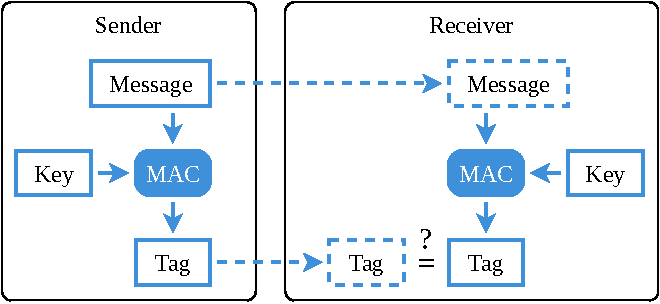
\includegraphics[width=0.6\linewidth]{figures/mac-structure.pdf}
    \caption{
        General structure of a \acrfull{mac}, where sender and receiver have a shared key. The
        receiver checks the output of the \acrshort{mac} to verify that the message was not modified
        in transit.
    }
    \label{fig:mac-structure}
\end{figure}

Inevitably, performing \acrshort{doa} on control messages would incur some computation and
communication overhead. Such latency is typically neglected when modeling, simulating, or
experimentally validating network protocols for quantum communications. In this work, we examine the
effects of latency caused by classical \acrshort{doa} on a simulated quantum network link requested
to generate entanglement between two nodes (henceforth referred to as the simulated quantum link).
First, we experimentally measure the latency incurred by a \acrshort{doa} system using
\acrshort{qkd}-powered authentication algorithms. We then analyze the behavior of the simulated
quantum link --- using a simulator for quantum networks~\cite{coopmans_2021_netsquid} --- where the
model of the control channel of the network includes the measured latencies incurred by the
\acrshort{qkd}-powered \acrshort{doa}. The contributions of this work are as follows:

\begin{enumerate}
    \item We provide a concise motivation for why \acrshort{doa} is a necessary component to uphold
          the availability of system-level protocols of the quantum network stack, and to help
          maintain the integrity of quantum data.
    \item We experimentally measure the added latencies incurred by \acrshort{doa}, performed using
          a \acrshort{qkd}-based authentication system, when run on a classical communication link.
    \item We offer a quantitative analysis of the impact of \acrshort{doa}, using the latencies
          measured as per the previous point, when applied to the quantum network protocols of a
          simulated quantum link (such link was first studied by \textcite{dahlberg_2019_egp}).
\end{enumerate}

\section{Related Work}
\label{sec:doa:relwork}

Conventional networking technology is an essential component of quantum networks and quantum
networking applications. \citeauthor{kozlowski_2019_towards} mention that the security of classical
communications is of concern when designing a quantum network~\cite{kozlowski_2019_towards}.
\citeauthor{satoh_2020_attacking} present a general motivation for authenticating the control
channel of a quantum link~\cite{satoh_2020_attacking}. They model attack vectors on quantum
communications through the lens of \acrfull{cia}. Without any security measures in place, an
attacker may:

\begin{itemize}
    \item Disrupt the network in any number of ways, affecting its \emph{availability}.
    \item Interfere with data sent via the network, hampering the \emph{integrity} of quantum data.
    \item Read out quantum data through the accompanying classical control data, affecting the
          \emph{confidentiality} of quantum data.
\end{itemize}

All identified proposals of quantum network designs and quantum network protocols use some form of
conventional communication to control and coordinate quantum
communication~\cite{van_meter_2013_repeaters, schoute_2016_shortcuts, joshi_2020_trusted,
pirker_2019_quantum, kozlowski_2019_towards, dahlberg_2019_egp, kozlowski_2020_qnp}. In this work,
we investigate one such proposal for a quantum network stack: the one put forth by
\textcite{dahlberg_2019_egp}, which has been evaluated in simulation, as well as on
hardware~\cite{pompili_2022_experimental}, and extended by \textcite{kozlowski_2020_qnp}.

The proposed protocol stack for quantum networks includes physical, link, network, transport, and
application layers, as illustrated in \cref{fig:functional-allocation}. The physical layer protocol,
called \acrfull{mhp}~\cite{dahlberg_2019_egp}, performs heralded entanglement generation attempts.
At the link layer, the \acrfull{qegp}~\cite{dahlberg_2019_egp} protocol has an internal retry
mechanism and performs coordination between adjacent nodes to provide more robust entanglement
generation. \acrshort{qegp} accepts two types of requests from the layer above:
%
\begin{inlinelist}
    \item \acrlong{ck} (\acrshort{ck}), to create an entangled pair and store it in memory;
    \item \acrlong{md} (\acrshort{md}), to create entangled pair, but measure it immediately, and
          report its outcome.
\end{inlinelist}
At the network layer, the \acrfull{qnp}~\cite{kozlowski_2020_qnp} protocol coordinates
entanglement generation and swap operations on a chain of nodes between two non-adjacent end nodes.

In this work, we simulate the three service-level protocols \acrshort{mhp}, \acrshort{qegp}, and
\acrshort{qnp}. In the next section, we explain why \acrfull{doa} is important for these protocols
to function, mostly focusing on \emph{availability} of the network and \emph{integrity} of quantum
data.

\section{Why Data Origin Authentication}
\label{sec:doa:why}

We investigate the applicability of \acrlong{doa} to three system-level protocols for quantum
network stacks: \acrshort{mhp}, \acrshort{qegp} and \acrshort{qnp}~\cite{dahlberg_2019_egp,
kozlowski_2020_qnp}. Quantum applications and their protocols themselves lie outside the scope of
this work. Here, we provide a non-exhaustive example list of actions that a malicious actor may
perform if they were able to forge or modify classical messages exchanged at the control protocol
level. We mention whether each action affects the \emph{availability} of the link or network, or the
\emph{integrity} of the quantum data sent via the network.

\paragraph{Physical layer}

\acrshort{mhp} operates at the physical layer. Hardware vulnerabilities of the physical entanglement
generation process are outside the scope of this work.

\begin{example}
\textit{Availability.}
Change a successful heralding signal to an error code such Alice and Bob falsely conclude that
entanglement has failed.
\end{example}

\begin{example}
\textit{Integrity.}
Modify a signal from a heralding station by changing the state announcement such that Alice or Bob
apply the wrong Pauli corrections to their qubits.
\end{example}

\begin{example}
\textit{Integrity.}
Interfere with mismatch verification~\cite{dahlberg_2019_egp, pompili_2022_experimental} such that
Alice and Bob falsely conclude that a \acrshort{mhp} request belongs to the same \acrshort{qegp}
request, thus hampering the integrity of quantum data due to cross-process interference.
\end{example}

\paragraph{Link layer}

\acrshort{qegp} operates at the link layer~\cite{dahlberg_2019_egp}. As proposed in
Ref.~\cite{dahlberg_2019_egp}, it is used to synchronize entanglement requests, and to communicate
the number of available memory qubits and the expiration of requests.

\begin{example}
\textit{Availability.}
Continually send requests for entanglement, exhausting the resources of nodes receiving
them~\cite{kozlowski_2019_towards}.
\end{example}

\begin{example}
\textit{Availability.}
When advertising the number of available communication qubits or storage qubits, set either to 0.
The receiving node then assumes that there are no communication or storage qubits available on the
sending node.
\end{example}

\begin{example}
\textit{Integrity.}
Change the qubit identifier of an entanglement generation request such that Alice and Bob entangle
the wrong data qubits, causing cross-path or process interference.
\end{example}

\paragraph{Network layer}

\acrshort{qnp} operates at the network layer. Conceptually, it allows non-adjacent nodes in a
quantum network to coordinate entanglement generation. This is akin to the \acrfull{ip} in the
classical stack. It makes use of \texttt{FORWARD} and \texttt{TRACK} messages to track entanglement
generation~\cite[Figure 6]{kozlowski_2020_qnp}. \texttt{FORWARD} messages are used to communicate
entanglement requests, and \texttt{TRACK} messages contain classical correction information for both
end-nodes in the network.

\begin{example}
\textit{Availability.}
Modify \texttt{FORWARD} message so that intermediary nodes do not receive entanglement swap
instructions.
\end{example}

\begin{example}
\textit{Integrity.}
Modify \texttt{TRACK} messages such that the end-nodes of a path do not receive the correct
entanglement swap outcome, and thus apply the wrong corrections to their qubits.
\end{example}

\begin{figure}[t]
    \centering
    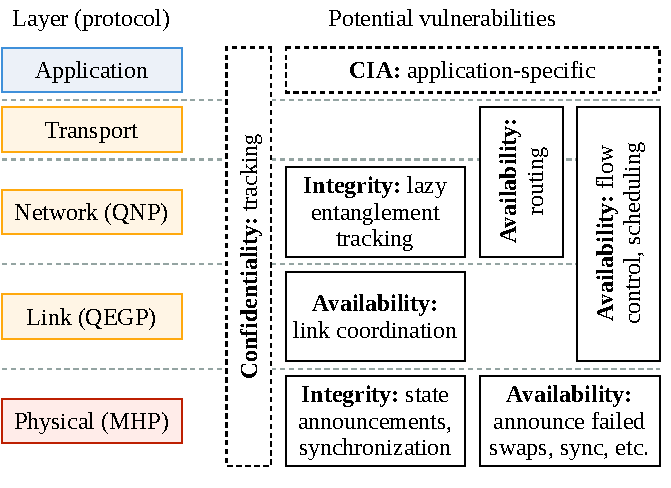
\includegraphics[width=0.6\linewidth]{figures/doa-examples.pdf}
    \caption{
        A summary of example effects of tampering with control messages at each layer of the quantum
        network stack through the lens of \acrfull{cia}. We take as examples concrete
        implementations of quantum network protocols --- including \acrshort{qnp}, \acrshort{qegp} and
        \acrshort{mhp}~\cite{kozlowski_2020_qnp, dahlberg_2019_egp} --- to highlight the
        potential vulnerabilities at each layer of the stack. In this work, we do not focus on
        confidentiality issues, as identified by \textcite{satoh_2020_attacking}.
    }
    \label{fig:doa-examples}
\end{figure}

We illustrate the concerns of availability and data integrity in a quantum network stack in
\cref{fig:doa-examples}. Such security threats are addressed in part by using \acrlong{doa}, which
can prevent modification and forgery of classical control messages. It should be noted, however,
that availability may still be hampered by an adversary capable of halting transmission of classical
control messages outright. Furthermore, if a malicious actor were to gain access to a node itself
then this might circumvent many or all security mechanisms in place, including \acrshort{doa}, and
should therefore also be prevented.

In general, we also note that classical control messages might reveal information about who is using
the network and the types of operations being performed. Therefore, in a more mature network, it
will likely be worthwhile to also encrypt the contents of control messages.
\textcite{satoh_2020_attacking} mention tracking as a general concern for inter-node classical
communication within the quantum stack. Encryption combined with transmission of random noise could
address tracking concerns.

\section{Experimental Methodology}
\label{sec:doa:meth}

We aim to examine the effects of \acrlong{doa}, and the total latency incurred by the classical
control messages, on the performance of a hypothetical quantum link. To limit the scope of our
investigation, we focus on the performance of link and physical layer protocols as proposed by
\textcite{dahlberg_2019_egp}, and we extend the simulation therein such that it fully captures
%
\begin{inlinelist}
    \item classical transmission overhead, roughly defined as the latency of classical messages
          through the network and all networking equipment, and
    \item \acrshort{doa} overhead, roughly defined as the processing time required by the
          \acrshort{doa} systems.
\end{inlinelist}

Instead of modeling transmission and authentication overhead analytically, we measure it
experimentally over a real-world, physically deployed network, consisting of multiple datacenter
locations, sample quantum node controllers running FreeRTOS~\cite{freertos} on a MicroZed
board~\cite{microzed}, and complete \acrshort{doa} servers. The \acrshort{doa} servers exist at both
ends of our real-world network, and run message authentication protocols. From a networking
perspective, these servers act like transparent proxy servers, and are thus generally unknown and
unseen to the quantum controllers, but do authenticate control messages between the two ends of our
real-world deployed network. The \acrshort{doa} servers authenticate (and validate) control messages
using key material obtained from a physically-deployed \acrshort{qkd} system, also running between
the datacenter locations. The \acrshort{qkd} devices form a \acrfull{mdiqkd} network, based on the
work by \textcite{berrevoets_2022_deployed}. The \acrshort{qkd} devices run next to the
\acrshort{doa} servers, and deliver \acrshort{qkd}-key material via standard interface protocols.

We recorded \acrfull{rtt} statistics of sample control messages sent between the quantum controllers
--- and thus through the message authentication protocols of the \acrshort{qkd}-powered
\acrshort{doa} servers. We then injected these \acrshort{rtt} data, along with other simulation
parameters described below, to extract metrics, as done in Ref.~\cite{dahlberg_2019_egp}, and assess
the performance of a simulated quantum entanglement generating link The measured control
communication overheads is reported in \cref{sec:doa:latency}, while the simulation results are
presented in \cref{sec:doa:results}.

\paragraph{\acrshort{doa} servers}

We collect control communication latency measurements under three different configurations of the
\acrshort{doa} servers:

\begin{enumerate}
    \item Bypass servers: at first, we bypass the \acrshort{doa} servers altogether. This is useful
          to measure baseline communication latency, excluding all computation delays that would be
          introduced by the servers.
    \item No \acrshort{mac}: this time, the \acrshort{doa} servers are configured to skip the
          authentication (and verification) step, but packets do go through the servers' processing
          pipelines. Results for this configuration give us insights into the overhead of processing
          packets on the \acrshort{doa} servers, excluding the computation latency incurred by the
          \acrshort{mac} authentication (and verification) step.
    \item \acrshort{poly}: finally, we configure the \acrshort{doa} servers to use
          \acrshort{poly}~\cite{bernstein_2005_poly1305}, which is a popular, fast, and
          computationally secure \acrshort{mac}. In this configuration, a \acrshort{doa} server
          attaches a \num{128}-bit mac to each outgoing message.
\end{enumerate}

We do not report on a configuration where the \acrshort{doa} servers use an
information-theoretically secure \acrshort{mac}, as such an authentication scheme would consume
considerably more key material than the \acrshort{qkd} system could deliver. We did verify this
assessment by configuring the \acrshort{doa} servers to use
\acrshort{vmac}~\cite{krovetz_2007_message} --- an information-theoretically secure \acrshort{mac}
--- during which the \acrshort{doa} servers attempted to use considerably more key material than
available.

\begin{figure}[t]
    \centering
    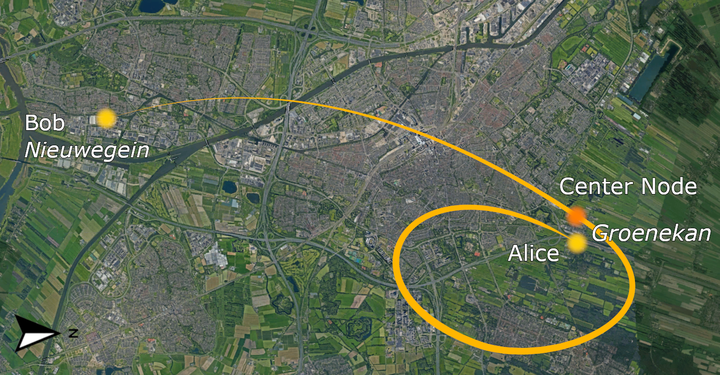
\includegraphics[width=0.6\linewidth]{figures/mac-setup-qkd-locations-resized.png}
    \caption{
        Physical layout of Alice and Bob nodes. Alice is located in Groenekan, the Netherlands,
        while Bob is in Nieuwegein, the Netherlands. The optical fiber connecting Alice to the
        center node is \qty{20}{\km} in length, whereas the connection between Bob and the center
        node is \qty{22}{\km}.
    }
    \label{fig:mac-setup-qkd-locations}
\end{figure}

\paragraph{Network topology}

In our network deployment, we name the two end locations Alice and Bob. As is normal in
\acrshort{mdiqkd}, each end location is connected to a center hub. In the real-world network, the
link connecting Alice to the center hub runs for \qty{20}{\km}, whereas the link between Bob and the
center hub is \qty{22}{\km} in length. Thus, the \acrshort{rtt} we measure is for a link of a total
length of \qty{42}{\km}. The topology of Alice, Bob, and the center hub of the \acrshort{mdiqkd}
system is illustrated in \cref{fig:mac-setup-qkd-locations}. The control communication overhead
measured in \cref{sec:doa:latency} will be scaled to simulate quantum links of various lengths
(\qtyrange{2.5}{75}{\km}) in \cref{sec:doa:results}.

\begin{figure}[t]
    \centering
    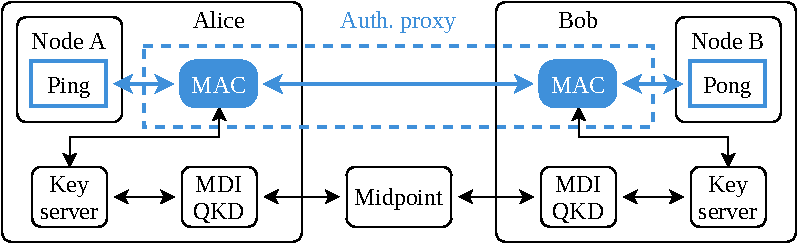
\includegraphics[width=0.6\linewidth]{figures/mac-setup-diagram.pdf}
    \caption{
        Experimental setup used to measure the end-to-end delays of transmitting an
        \emph{authenticated classical message} from Alice to Bob with \qty{42}{\km} of fiber-optic
        cables between them. Classical messages go through a \acrshort{doa} server that tags
        messages using \acrshort{mdiqkd}-generated key material.
    }
    \label{fig:mac-setup-diagram}
\end{figure}

\section{Classical Communication Latency}
\label{sec:doa:latency}

In order to obtain an estimate of the expected latency incurred by classical control messages in a
quantum network stack, we measure the \acrfull{rtt} of a sample of messages when sent through an
authenticated classical channel in the field. The messages are \acrshort{icmp} (ping) packets, sized
to mimic \acrshort{mhp} and \acrshort{qegp} packets. The authentication mechanism is external to the
controllers exchanging ping messages, and runs on transparent \acrshort{doa} proxy servers between
them. The \acrshort{doa} server next to the sender calculates a \acrshort{mac} tag over the sent
message, forwards the message and the tag to the receiver, whose \acrshort{doa} servers verifies the
tag before delivering the message to the destination controller. The experimental setup is depicted
in \cref{fig:mac-setup-diagram}.

Ping messages are exchanged between two real-time classical network nodes similar to those used in
the experimental validation of \acrshort{qegp}~\cite{pompili_2022_experimental} --- MicroZed
boards~\cite{microzed} running a FreeRTOS~\cite{freertos} application --- connected to the
\acrshort{doa} servers via Gigabit Ethernet interfaces. The sending node records the \acrshort{rtt}
of the message, and computes various statistics on these timestamps, most notably average and
standard deviation. We use these statistics to extrapolate the expected control communication
latency for the various quantum link simulation scenarios presented in \cref{sec:doa:results}.

The \acrfull{mac} on both ends retrieves authentication keys from a local \acrshort{qkd} node
running a \acrshort{qkd} key server, which contains key material identical to its counterpart at the
other end. Key material is produced by an \acrshort{mdiqkd} implementation deployed in the Utrecht
area, in the Netherlands. The \acrshort{mdiqkd} system is very similar to the one implemented in
Ref.~\cite{berrevoets_2022_deployed}.

\paragraph{Rate and size of messages}

When using our particular \acrshort{doa} servers, one cannot transmit a classical message more than
once every \qty{10}{\ms} without experiencing detrimental packet loss. The reason for this is that
the \acrshort{doa} servers run prototype software designed for research purposes, and have not been
optimized for performance. We thus transmit ping messages at a rate of \qty{100}{\Hz}. Moreover, the
employed \acrshort{doa} servers can only authenticate packets with a payload that is small enough to
be accommodated (together with all protocol headers and the \acrshort{mac} tag) in a single Ethernet
frame. Therefore, we send ping messages with payloads of
%
\begin{inlinelist}
    \item \num{12}~bytes, which is the size of the smallest \acrshort{qegp} message, and
    \item \num{1200}~bytes, which is close to the maximum allowed by the \acrshort{doa} server.
\end{inlinelist}
The second configuration is useful to examine how much \acrshortpl{rtt} depend on the size of the
message.

\paragraph{Results}

We record the \acrlong{rtt} of 360,000 ping messages per configuration (\acrshort{doa} server
configuration and size of message). Mean and standard deviation of the measured \acrshortpl{rtt} are
reported in \cref{tab:rtt}, whilst the raw distributions of \acrshort{rtt} measurements are
presented in \cref{app:rtt}.

When bypassing the \acrshort{doa} servers altogether, \acrshort{rtt} delays follow a simple Gaussian
distribution, with a mean of less than \qty{4}{\ms} and a standard deviation of around
\qty{20}{\us}. When messages go through the \acrshort{doa} servers (configurations ``No
\acrshort{mac}'' and ``\acrshort{poly}''), \acrshort{rtt} measurements can be approximated by
bimodal Gaussian distributions (see \cref{app:rtt}). This bimodal distribution is likely the result
of some caching behavior exhibited by the \acrshort{doa} servers. For both configurations, one of
the two modes strongly dominates over the other, with the mean of this mode (around \qty{14}{\ms}
for all configurations and sizes) being approximately equal to the overall mean of the entire
distribution ($\pm\qty{2}{\percent}$ difference at most). \Cref{tab:rtt} reports mean and standard
deviation of the strongest modes of each distribution, which are deemed to be the most
representative statistics to use in our simulations. Refer to \cref{app:rtt} for a more in-depth
analysis of the \acrshort{rtt} distributions.

The noticeable gap between ``Bypass servers'' and the other two configurations is an indicator of
the suboptimal packet processing performance of the \acrshort{doa} server, which is merely a
soft-processing packet pipeline implemented in Python. The computational overhead introduced by the
actual \acrshort{mac} is overshadowed by the baseline latency of the \acrshort{doa} servers, as
observed in the ``\acrshort{poly}'' configuration. Interestingly, the size of messages does not
appear to be a noticeable factor in the mean end-to-end latency.

\begin{table}
    \centering
    \begin{tabularx}{0.75\linewidth}{@{} lYYYY @{}}
        \toprule
        \textbf{Server}                    & \textbf{Payload} & \multicolumn{2}{c}{\textbf{\acrshort{rtt}} [\unit{\us}]}                \\
        \cmidrule(l){3-4}
        \textbf{configuration}             & [Bytes]          & \textbf{mean}                                            & \textbf{std} \\
        \midrule
        \multirow{2}{*}{Bypass servers}    & \num{12}         & \num{3657}                                               & \num{23}     \\
                                           & \num{1200}       & \num{3881}                                               & \num{22}     \\
        \midrule
        \multirow{2}{*}{No \acrshort{mac}} & \num{12}         & \num{14036}                                              & \num{797}    \\
                                           & \num{1200}       & \num{14089}                                              & \num{767}    \\
        \midrule
        \multirow{2}{*}{\acrshort{poly}}   & \num{12}         & \num{14099}                                              & \num{861}    \\
                                           & \num{1200}       & \num{14015}                                              & \num{729}    \\
        \bottomrule
    \end{tabularx}
    \caption{
        Mean and standard deviation of \acrfull{rtt} for different configurations of the
        \acrshort{doa} servers and for different message sizes. Measurements for the ``Bypass
        servers'' configuration follow a simple Gaussian distribution. Measurements for the other
        two configurations can be approximated by bimodal Gaussian distributions, with one of the
        two modes strongly dominating over the other. This table reports mean and standard deviation
        of the strongest modes of each distribution. In the ``\acrshort{poly}'' configuration, the
        \acrshort{doa} servers attaches a \num{128}-bit key to each message.
    }
    \label{tab:rtt}
\end{table}

We can therefore conclude that latency is dominated by two main factors:
%
\begin{inlinelist}
    \item the performance of any classical networking hardware and the length of the classical link,
          which depend on the network technology and topology, and
    \item the packet processing performance of the \acrshort{doa} servers.
\end{inlinelist}
However, in a real production network, it is fair to assume that packets will be processed at a much
faster rate, and thus result in an end-to-end latency that is much more similar to that of the
``Bypass servers'' configuration. Considering also that authentication does not incur any noticeable
overhead --- as shown by the difference between the ``No \acrshort{mac}'' and ``\acrshort{poly}''
configurations --- these results support the case for both the use of \acrshort{doa} in quantum
networks, as well as the use of \acrshort{doa} supported by \acrshort{qkd} in present-day,
real-world production networks.

\section{Simulation Results}
\label{sec:doa:results}

We quantify the effects of using an authenticated classical channel for control messages exchanged
at the quantum network stack level. In particular, we augment the model used by
\textcite{dahlberg_2019_egp} to simulate the performance of physical (\acrshort{mhp}) and link
(\acrshort{qegp}) layer control protocols within the quantum network stack. As opposed to the
original work, we model the classical control communication latency to also include transmission and
authentication overhead as experimentally measured in our real-world network, and presented in
\cref{sec:doa:latency}. We report the \emph{throughput} of the quantum link, expressed as number of
entangled pairs generated per second.

We use \acrshort{rtt} statistics from \cref{tab:rtt} for our simulations. As described in
\cref{sec:doa:latency}, \acrshort{rtt} measurements for the ``Bypass servers'' configuration can be
approximated by a Gaussian distribution. \acrshortpl{rtt} for the ``No \acrshort{mac}'' and
``\acrshort{poly}'' configurations instead follow bimodal Gaussian distributions, with one of the
modes dominating over the other. For these two configurations, we use mean and standard deviation of
the strongest mode.

\paragraph{Configurations}

We run our simulations for two types of configurations:
%
\begin{inlinelist}
    \item To begin with, we analyze the quantum link throughput for several node-to-node distances
          (\qtyrange{2.5}{75}{\km}), at a fixed requested fidelity ($F_\text{min}=0.65$). For the
          various distances, we scale the classical delays measured in \cref{sec:doa:latency}
          accordingly. For this configuration, we compare our augmented model with the original
          baseline, in which transmission and authentication delays were not
          modeled~\cite{dahlberg_2019_egp}.
    \item Furthermore, we analyze the quantum link throughput at a fixed node-to-node distance
          (\qty{42}{\km} between the two nodes, same as in the real-world network in
          \cref{sec:doa:latency}), but this time varying the requested fidelity at the
          \acrshort{qegp} layer (fidelity \numrange{0.50}{0.85}). This time, we compare three
          models, corresponding to the three configurations of the \acrshort{doa} servers as per
          \cref{sec:doa:latency}: ``Bypass servers'', ``No \acrshort{mac}'', and
          ``\acrshort{poly}''.
\end{inlinelist}

For each of the above configurations, we perform \num{20} simulation runs, each consisting of
\num{20} minutes of continuous use of the quantum link. We then calculate the average throughput
over all runs for each configuration with a confidence interval of \qty{95}{\percent}.

\paragraph{Results}

\begin{figure}[t]
    \centering
    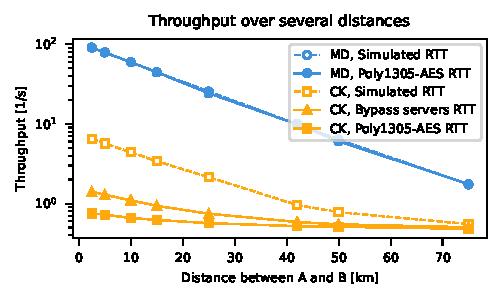
\includegraphics[width=0.6\linewidth]{figures/throughput-vs-distance.pdf}
    \begin{tabularx}{0.6\linewidth}{@{} lYYYYYYYY @{}}
        \toprule%
                        & \multicolumn{8}{c}{\textbf{Breakdown of distance A -- B [\unit{\km}]}}                                   \\%
        \midrule%
        \textbf{A -- M} & 1.5                                                                    & 3 & 6  & 9  & 15 & 22 & 30 & 45 \\%
        \textbf{M -- B} & 1                                                                      & 2 & 4  & 6  & 10 & 20 & 20 & 30 \\%
        \midrule%
        \textbf{Total}  & 2.5                                                                    & 5 & 10 & 15 & 25 & 42 & 50 & 75 \\%
        \bottomrule                             %
    \end{tabularx}%
    \caption{
        Throughput (rate) of entangled pair generation for multiple distances between node A and B,
        with a single midpoint station in between and for a requested fidelity of
        $F_\text{min}=0.65$. Classical communication delays were modeled using latency measurements
        collected as described in \cref{sec:doa:latency} --- configurations ``Bypass servers'' and
        ``\acrshort{poly}'' --- as well as replicated from the original simulations of \acrshort{qegp}
        and \acrshort{mhp}~\cite{dahlberg_2019_egp}. The simulated \acrshort{rtt} configuration
        represents the best-case scenario, given that only propagation delays are modeled in this
        one. The configuration ``\acrshort{poly}'' is the worst-case scenario instead, given that it
        models delays measured on the field, including the overhead incurred by the slow packet
        processing pipeline. For \acrshort{md} type requests, only the best case and the worst case
        are plotted, since they practically overlap, and thus any other scenario in between best and
        worst would not result in any significant difference. The table below the plot shows how
        distance is distributed between A, B, and the midpoint station M. The \qty{25}{\km} data
        point is equivalent to the QL2020 hypothetical setup simulated in
        Ref.~\cite{dahlberg_2019_egp}.
    }
    \label{fig:results-distance}
\end{figure}

The results for throughput versus distance are illustrated in \cref{fig:results-distance}. For
\acrfull{md} type requests (for which entanglement can be measured directly, as described in
earlier), mean throughput is approximately equal across the two models of added latency. This is to
be expected, given that these types of requests can be effectively pipelined --- that is, the next
entanglement request can be initiated right after the previous one without the need to wait for any
acknowledgment messages from a heralding station --- and thus throughput is mostly dominated by the
physical entanglement generation procedure, and not as much by classical communication latency. On
the other hand, \acrfull{ck} requests (for which entanglement must be stored while waiting for
acknowledgment messages, as described earlier) show a variation in throughput that depends on the
delay model. The best-case scenario --- corresponding to the original simulations of \acrshort{mhp}
and \acrshort{qegp}~\cite{dahlberg_2019_egp} (``Simulated RTT'') --- results in the highest
throughput, which peaks at around \num{6.47} pairs per second at the shortest distance. This is
followed by the scenario with ``Bypass servers'' delays, where classical communication latency has a
higher overhead than the previous case, but is more realistic. In this case, the shortest link can
deliver around \num{1.42} entangled pairs per second. Finally, the worst-case scenario of
``\acrshort{poly}'', where classical communication delays also include the overhead of the slow
packet processing pipeline of the \acrshort{doa} servers, can yield a little less than one pair per
second. This decrease in throughput is expected, but fortunately, it is also not detrimental to the
point that the quantum link becomes non-functional altogether. Naturally, final numbers depend
strongly on the quantum properties of the quantum memories (quantum coherence time). Conceivably, if
the coherence time of the quantum memories was longer than the added latency of \acrshort{doa}
servers, the decrease in performance would be less significant.

The results for throughput versus fidelity are shown in \cref{fig:results-fidelity}. Again, the
outcome matches our expectations. \acrshort{md} requests are not significantly affected by classical
communication, and their throughput only decreases when higher-fidelity entangled pairs are
requested. \acrshort{ck} requests, instead, are more affected by classical communication latency,
and their throughput is a lot lower than that of \acrshort{md} requests. Additionally, throughput
also decreases when classical messages go through the \acrshort{doa} servers (``Bypass servers''
versus ``No \acrshort{mac}''). As expected from the results in \cref{tab:rtt}, the extra latency
incurred by the actual \acrshort{mac} computation are negligible, and its effect on throughput not
noticeable (``No \acrshort{mac}'' versus ``\acrshort{poly}'').

\begin{figure}[t]
    \centering
    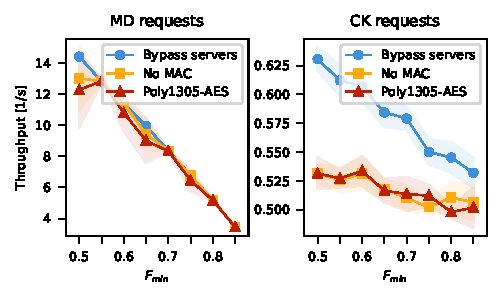
\includegraphics[width=0.6\linewidth]{figures/throughput-vs-fidelity.pdf}
    \caption{
        Throughput (rate) of entangled pair generation for multiple requested fidelities, with
        \qty{20}{\km} between node A and the midpoint station, and \qty{22}{\km} between the
        midpoint station and node B, and for three configurations of the proxy as per
        \cref{sec:doa:latency}: Bypass servers, No \acrshort{mac}, and \acrshort{poly}. The solid line
        represents mean throughput, the colored area around it depicts the \qty{95}{\percent}
        confidence interval. \Acrfull{md} type requests are not as heavily affected as these are
        pipelined. \Acrfull{ck} type requests are performed sequentially, and thus increases in
        classical delays have a more profound impact on throughput.
    }
    \label{fig:results-fidelity}
\end{figure}

To summarize, our experiments and simulations demonstrate that
%
\begin{inlinelist}
    \item in real-world quantum links, throughput is likely to be worse than what results from
          simulations that do not fully model transmission delays of messages stemming from
          latencies of conventional communication networks,
    \item the overhead incurred by classical communications is sizeable, but does not outright
          disrupt the operation of quantum links, and
    \item delays incurred by \acrlong{doa} are negligible.
\end{inlinelist}

\section{Discussion}

We have shown how the classical data plane of a quantum network stack presents a significant attack
surface for \acrlong{cia} of the quantum link and data therein. To address these concerns one must
employ, among other things, \acrlong{doa} on the classical control messages exchanged at the quantum
network stack level. We conclude that \acrlong{doa} is necessary to both uphold the integrity of
quantum data and the availability of the quantum network itself.

We have also simulated the performance of a hypothetical quantum link under the assumption that
control messages are authenticated by conventional \acrshort{doa} techniques. Here, we modeled
classical communication latency, including authentication overhead and transmission delay, using
metrics collected from a real-world communication link, authenticated using \acrshort{doa} servers,
using key material sourced from a \acrshort{qkd} system. If we disregard the large packet processing
delays incurred by the \acrshort{doa} servers itself --- the delays of the servers packet pipeline,
and not the delays of the authentication software running on the server --- we observe that an
authenticated classical control channel introduces a negligible amount of extra classical overhead.

However, we have also seen that even just transmission delays have a noticeable effect on the
performance of a quantum link, whether or not \acrlong{doa} is applied --- entanglement generation
throughput drops when classical communication delays are larger. Nevertheless, we have observed in
our simulations that even when the entangled qubits must be stored in quantum memories with limited
lifetimes, the quantum link remains operational.

\begin{xstretch}
\printbibliography[heading=subbibintoc,title={References},notcategory=noprint]
\end{xstretch}
